% !TEX root = ../main.tex
% Бүлэг 5

\chapter{Загвар хөгжүүлэлт ба туршилтын үр дүн}
\label{Chapter5}
\pagecolor{Beige}

Энэ бүлэгт судалгааны явцад боловсруулсан загваруудын хөгжүүлэлт, сургалтын орчин, туршилтын тохиргоо болон үр дүнг танилцуулна. Мөн судалгааны явцад хэрэгжүүлсэн гурван өөр туршилтын аргын гүйцэтгэлийг харьцуулан шинжилж, эцсийн байдлаар сонгосон pipeline-ийн давуу талыг тодорхойлов.

%───────────────────────────────────────────────────────────────────────────────
\section{Суурь загвар ба үнэлгээний хэмжүүрүүд}

Санал болгож буй аргын үр нөлөөг үнэлэхийн тулд хэд хэдэн суурь загвар (baseline model)-тай харьцуулсан. Ангиллын даалгаварт ConvNeXt-Small болон EfficientNet-B3 архитектуруудыг ашигласан бол сегментчлэлийн даалгаварт U-Net загварыг суурь загвар болгон сонгов. Эдгээр архитектурууд нь эмнэлгийн дүрс боловсруулалтын судалгаанд өргөн хэрэглэгддэг бөгөөд өмнөх судалгааны үр дүнтэй харьцуулах боломж олгодог.

Загваруудын гүйцэтгэлийг даалгавар тус бүрт тохирсон үнэлгээний хэмжүүрүүдээр үнэлэв. Ангиллын даалгаварт Accuracy, Precision, Recall, F1-score болон AUC үзүүлэлтүүдийг ашигласан. Сегментчлэлийн чанарыг Dice coefficient болон Intersection over Union (IoU)-оор үнэлсэн. Хугарлын зэргийн үнэлгээнд Exact болон Adjacent accuracy ($|\hat{y}-y|\leq1$)-ийг, харин эдгэрэлтийн үнэлгээний модульд Mean Absolute Error (MAE), Root Mean Square Error (RMSE) болон $R^2$ үзүүлэлтүүдийг ашиглав.

Хүснэгт~\ref{tab:metrics}-д судалгаанд ашигласан үндсэн үнэлгээний хэмжүүрүүдийг харуулав.

\begin{table}[!htbp]
\centering
\small
\begin{tabular}{l l l}
\toprule
\textbf{Даалгавар} & \textbf{Хэмжүүр} & \textbf{Тодорхойлолт / томьёо} \\
\midrule
\multirow{5}{*}{Ангилал}
  & Accuracy  & $(TP+TN)/(TP+TN+FP+FN)$ \\[2pt]
  & Precision & $TP/(TP+FP)$ \\[2pt]
  & Recall    & $TP/(TP+FN)$ \\[2pt]
  & F1-score  & $2\cdot P\cdot R/(P+R)$ \\[2pt]
  & AUC-ROC   & ROC муруйн доорх талбай \\[4pt]
\multirow{2}{*}{Сегментаци}
  & Dice & $2|A\cap B| / (|A|+|B|)$ \\[2pt]
  & IoU  & $|A\cap B| / |A\cup B|$ \\[4pt]
\multirow{2}{*}{Хугарлын зэрэг}
  & Exact Accuracy    & Зэрэглэлийг яг таарсан хувь \\[2pt]
  & Adjacent Accuracy & $|\hat{y}-y|\leq 1$ байх хувь \\[4pt]
\multirow{3}{*}{Эдгэрэлт}
  & MAE  & $\frac{1}{n}\sum|\hat{y}_i-y_i|$ \\[2pt]
  & RMSE & $\sqrt{\frac{1}{n}\sum(\hat{y}_i-y_i)^2}$ \\[2pt]
  & $R^2$ & $1-\mathrm{SS_{res}}/\mathrm{SS_{tot}}$ \\
\bottomrule
\end{tabular}
\caption{Судалгаанд ашигласан үнэлгээний хэмжүүрүүд}
\label{tab:metrics}
\end{table}

%───────────────────────────────────────────────────────────────────────────────
\section{Санал болгож буй архитектур}

Энэхүү судалгаанд ясны хугарлын рентген зураг боловсруулах дөрвөн үе шаттай модульчлагдсан pipeline санал болгосон. Pipeline нь хугарал илрүүлэх, сегментлэх, хугарлын зэргийг үнэлэх болон эдгэрэлтийн төлөвийг таамаглах гэсэн дараалсан бүрэлдэхүүн хэсгүүдээс бүрдэнэ.

Эхний шатанд рентген зураг ангиллын модульд орж хугарал байгаа эсэхийг тодорхойлно. Хугарал илэрсэн тохиолдолд сегментчлэлийн модуль хугарлын бүсийг пиксел түвшинд ялган гаргана. Үүний дараа сегментчлэлийн үр дүнд үндэслэн хугарлын геометрийн шинжүүдийг тооцоолж, хугарлын зэргийг үнэлнэ. Эцэст нь гаргаж авсан шинжүүдийг ашиглан эдгэрэлтийн төлөвийг таамаглана.

Ангиллын модульд ConvNeXt архитектур (эцсийн pipeline-д ImageNet-22K урьдчилсан сургалттай ConvNeXt-Base), сегментчлэлийн модульд эрлийз ResNet50 U-Net, хугарлын зэрэг үнэлэх хэсэгт морфологийн шинжүүдэд суурилсан proof-of-concept үнэлгээний арга, эдгэрэлтийн модульд синтетик клиникийн өгөгдөл дээр туршсан proof-of-concept регрессийн загварыг ашиглав.

ConvNeXt-Base-ийг эцсийн ангиллын модулиар сонгосон нь зөвхөн гүйцэтгэлийн тоон үзүүлэлттэй холбоотой биш юм. Рентген зураг дахь хугарал нь ихэвчлэн нарийн шугам, ирмэгийн тасралт, ясны хэлбэрийн бага хэмжээний өөрчлөлт байдлаар илэрдэг тул загвар орон зайн локал шинжийг алдалгүй хадгалах шаардлагатай. ConvNeXt нь convolution-д суурилсан архитектур хэвээр боловч том kernel бүхий depthwise convolution, LayerNorm, GELU болон Transformer-тэй төстэй блокийн зохион байгуулалтыг ашигладаг тул локал болон өндөр түвшний дүрслэлийн шинжийг зэрэг сурах давуу талтай.

Өгөгдлийн талаас авч үзвэл эцсийн ангиллын сургалт нь олон эх сурвалжийн рентген зургаас бүрдсэн. Ийм нөхцөлд нэг өгөгдлийн сангийн дүрсний хэв шинжид хэт тохирохоос сэргийлэхийн тулд ImageNet-22K дээр урьдчилан сурсан илүү өргөн төлөөлөлтэй backbone ашиглах нь зүйтэй гэж үзсэн. ConvNeXt-Base нь ConvNeXt-Small, EfficientNet-B3 болон ResNet-50 загваруудтай харьцуулахад параметрийн хувьд том боловч RTX A6000 серверийн нөөцөд багтаж, тестийн үед хамгийн өндөр ялгах чадвар үзүүлсэн.

Мөн ConvNeXt-Base сонголт нь pipeline-ийн эхний шатны ач холбогдолтой холбоотой. Ангиллын модуль буруу сөрөг гаргавал дараагийн сегментчлэл, хугарлын зэрэг болон эдгэрэлтийн модулиуд огт ажиллахгүй. Иймээс эхний шүүлтүүрийн recall болон AUC өндөр байх нь нийт pipeline-ийн найдвартай ажиллагаанд шууд нөлөөлнө. Энэ шалтгаанаар эцсийн pipeline-д илүү хөнгөн загвараас илүү өндөр гүйцэтгэлтэй ConvNeXt-Base хувилбарыг сонгосон.

Зураг~\ref{fig:proposed_arch}-д санал болгож буй архитектурын ерөнхий бүтцийг үзүүлэв.

\begin{figure}[!htbp]
\centering
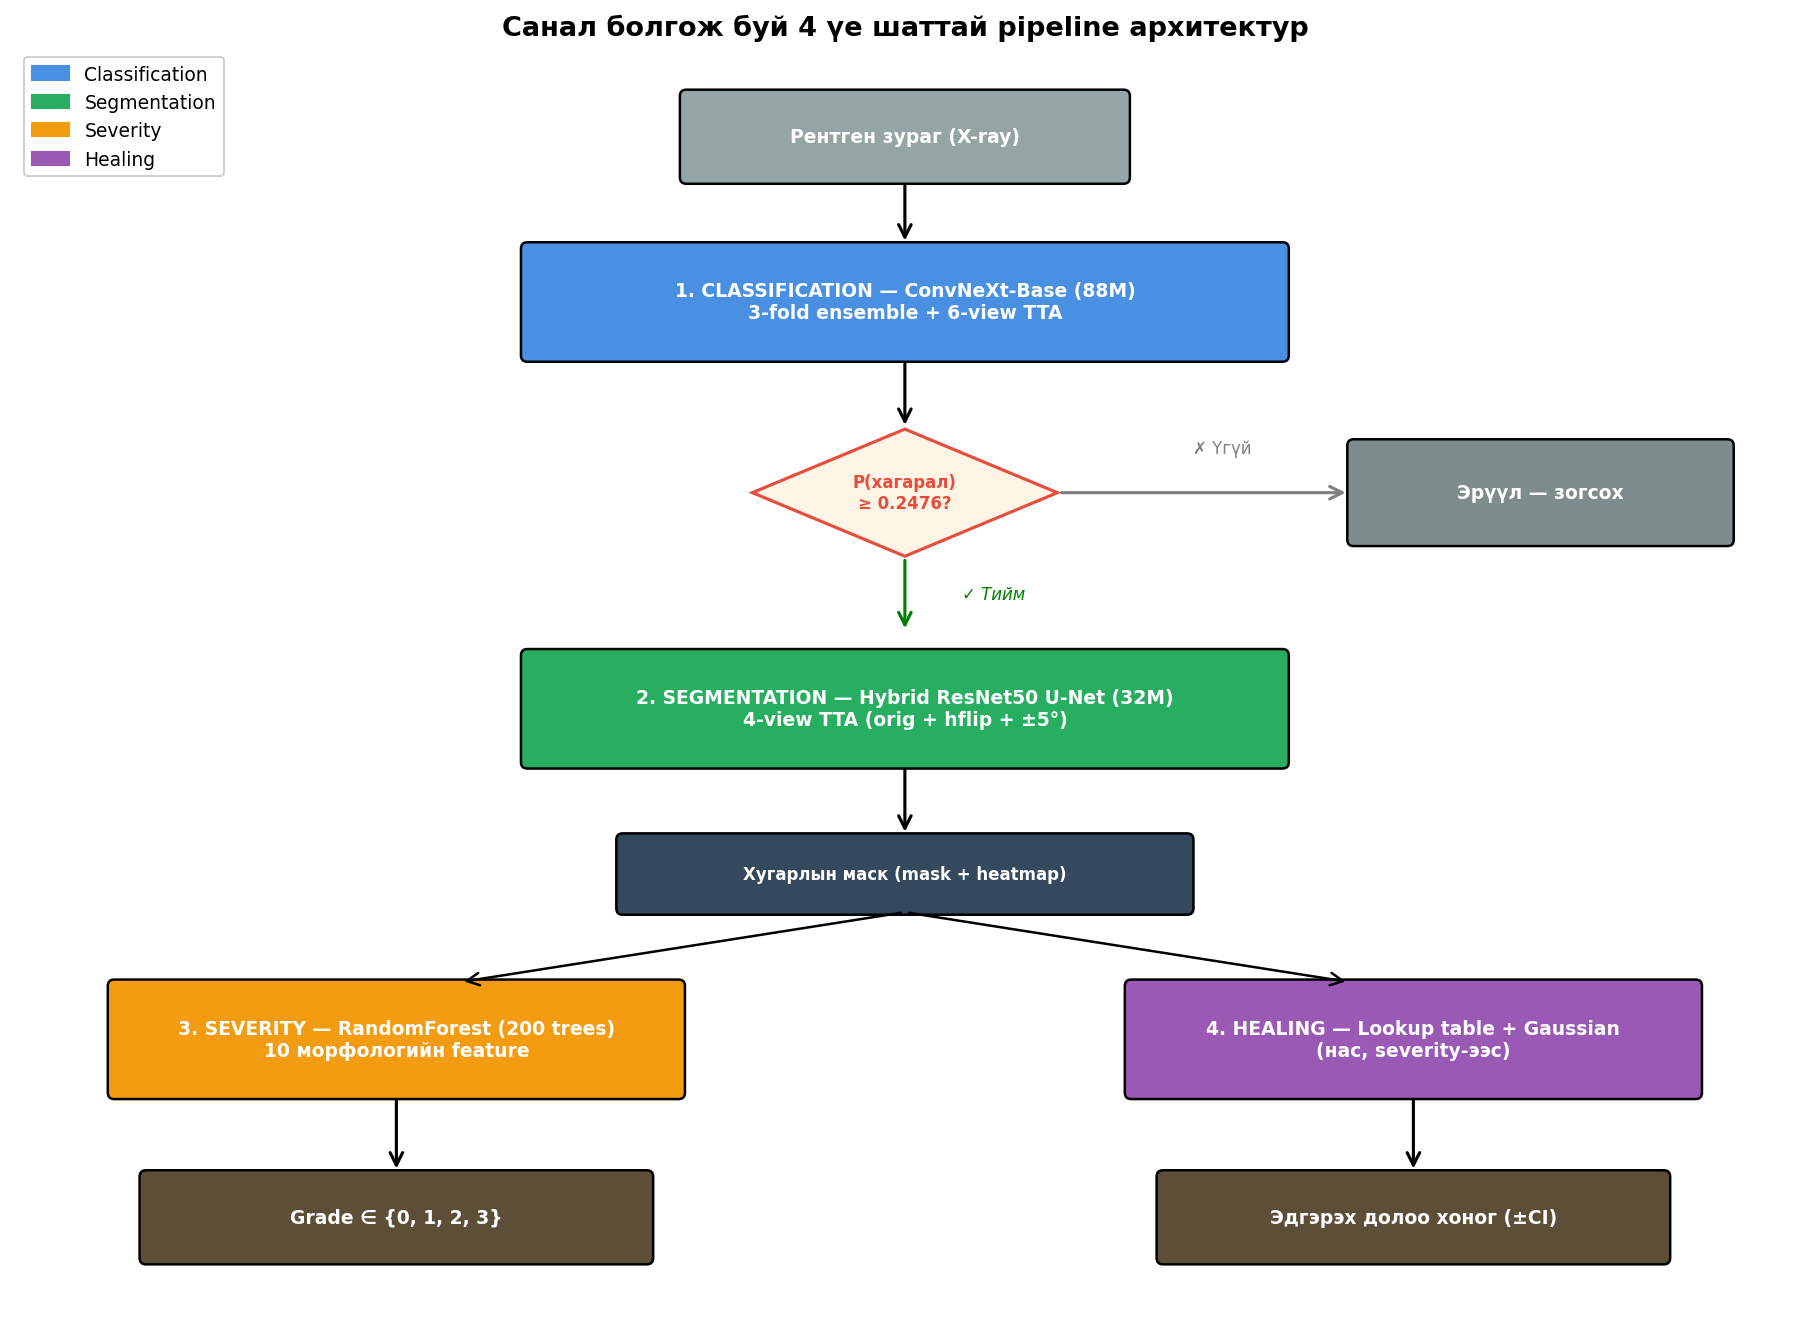
\includegraphics[width=\textwidth]{Figures/Figure_5_1.png}
\figcaption{Санал болгож буй pipeline архитектур}{Санал болгож буй дөрвөн үе шаттай модульчлагдсан pipeline архитектур}
\label{fig:proposed_arch}
\end{figure}

%───────────────────────────────────────────────────────────────────────────────
\section{Сургалтын pipeline}

Сургалтын pipeline нь өгөгдөл цуглуулах, урьдчилан боловсруулах, загвар сургах, үнэлэх болон үр дүнг тайлбарлах гэсэн үндсэн үе шатуудаас бүрдэнэ.

Эхний хоёр туршилтад MURA өгөгдлийн санг ангиллын суурь сургалтад ашигласан. Харин эцсийн буюу гурав дахь туршилтын ангиллын модульд GRAZPEDWRI-DX, FracAtlas-COCO, YOLOBoneFracture болон BoneFractureCVProject өгөгдлийн сангуудыг нэгтгэн ашиглав. FracAtlas өгөгдлийг эцсийн pipeline-д голчлон сегментчлэл болон хугарлын зэргийн үнэлгээнд хэрэглэсэн. Өгөгдлийг сургалт, баталгаажуулалт болон тестийн багцуудад хувааж, дүрсийн хэмжээг нэгэн жигд болгож, нормчлол болон өгөгдөл нэмэгдүүлэх аргуудыг хэрэгжүүлэв.

Үүний дараа ангилал болон сегментчлэлийн загваруудыг тус тус сургаж, үр дүнг баталгаажуулалтын өгөгдлөөр үнэлэв. Хугарлын зэрэг болон эдгэрэлтийн үнэлгээний модулиуд нь өмнөх үе шатуудаас гарсан үр дүнг ашиглан ажиллана.

Зураг~\ref{fig:training_pipeline}-т сургалтын ерөнхий pipeline-ийг харуулав.

\begin{figure}[!htbp]
\centering
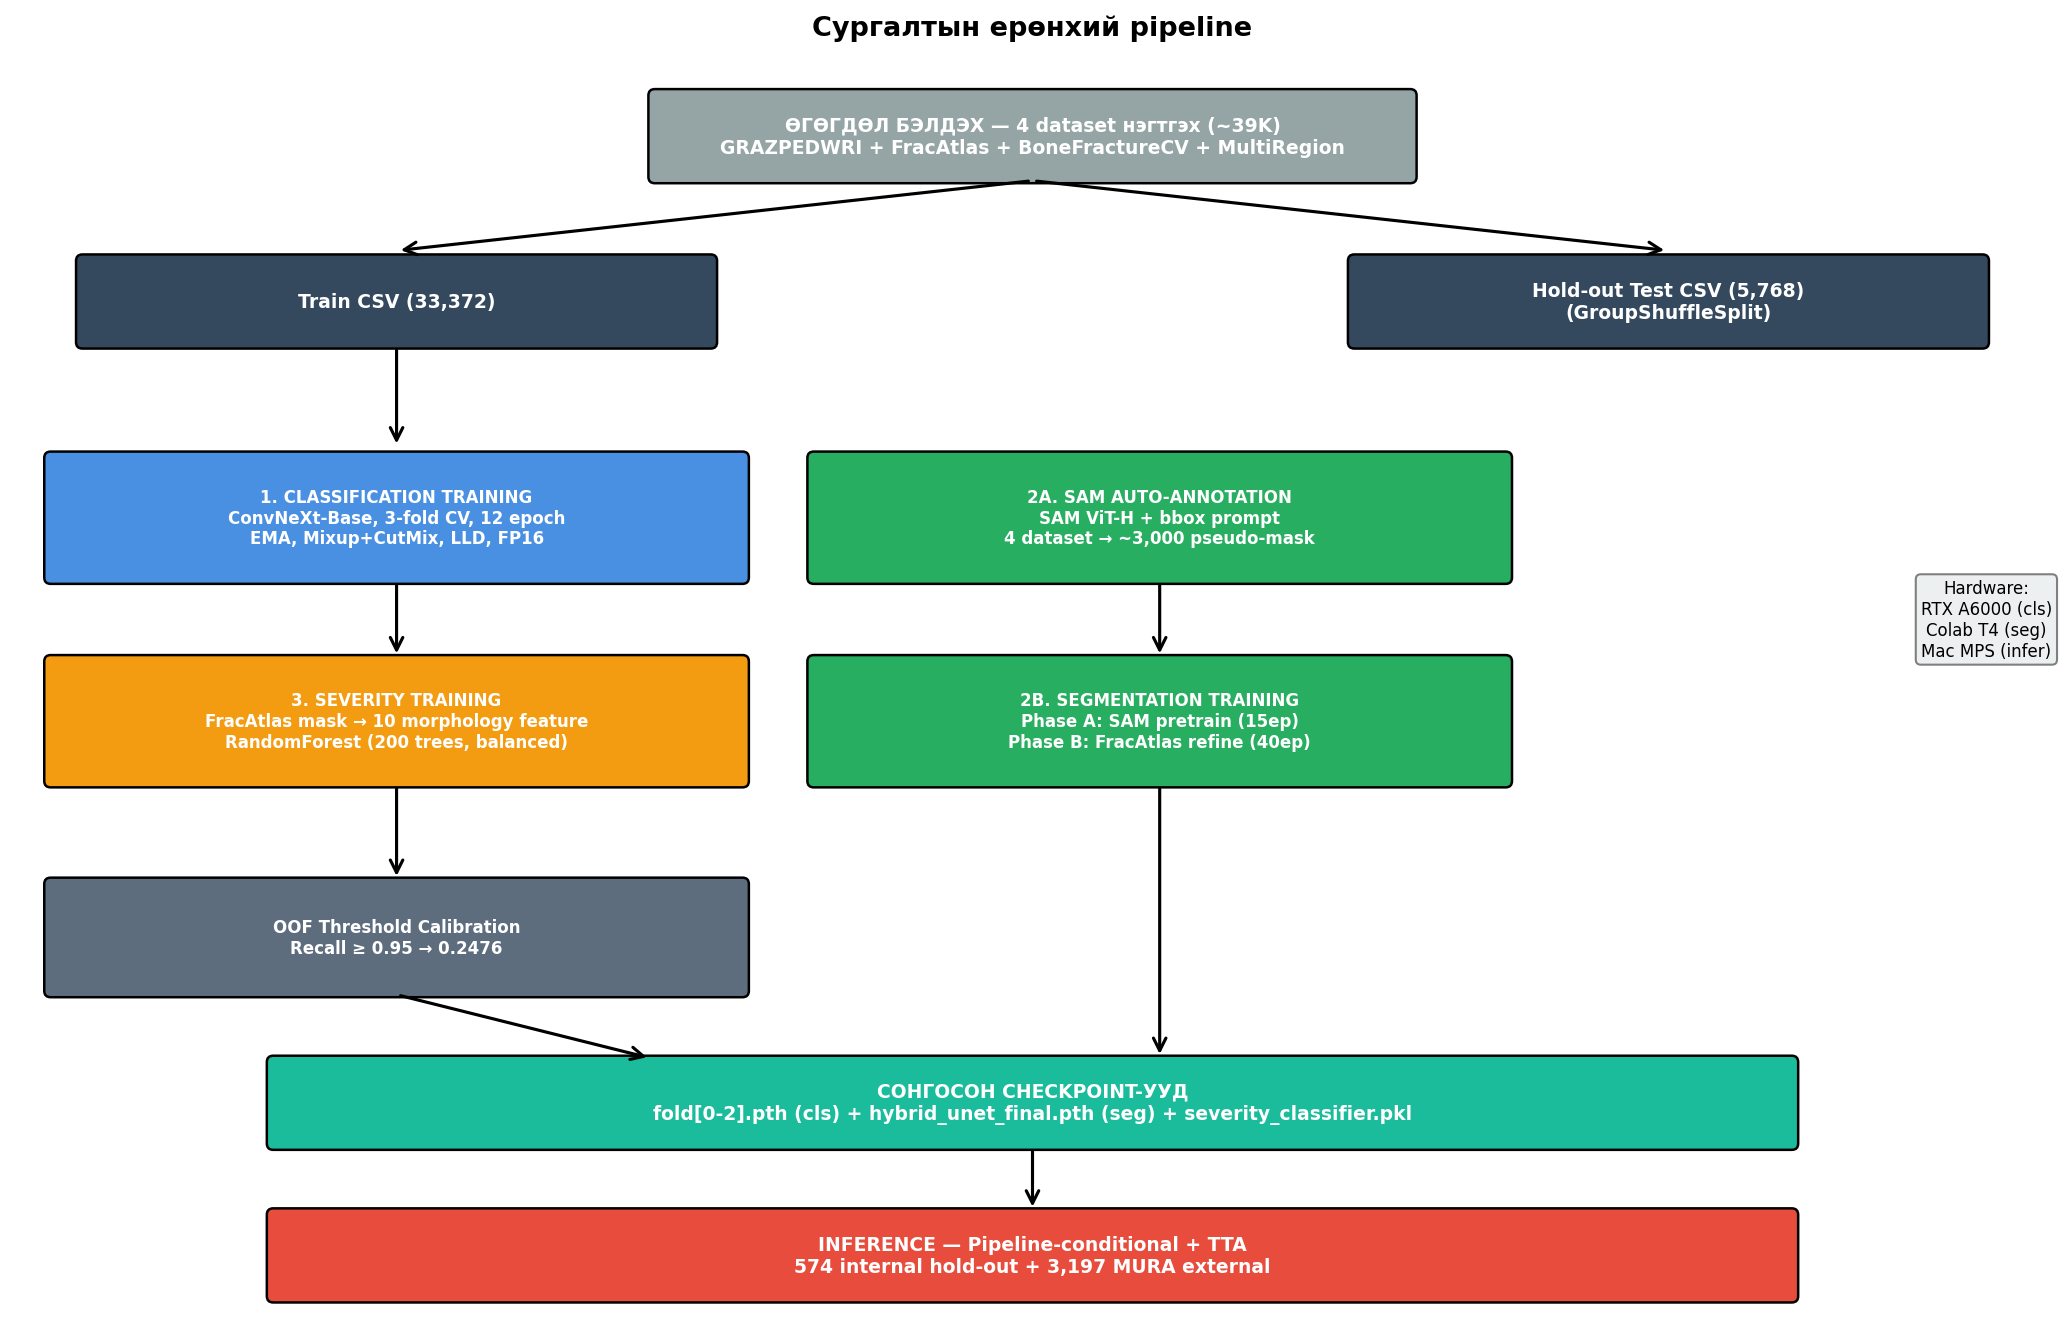
\includegraphics[width=\textwidth]{Figures/Figure_5_2.png}
\figcaption{Сургалтын ерөнхий pipeline}{Сургалтын ерөнхий pipeline — өгөгдөл цуглуулах, урьдчилан боловсруулах, загвар сургах, үнэлэх болон үр дүнг тайлбарлах үндсэн үе шатууд}
\label{fig:training_pipeline}
\end{figure}

%───────────────────────────────────────────────────────────────────────────────
\section{Туршилтын тохиргоо}

Туршилтын орчныг даалгаврын тооцооллын шаардлагаас хамааруулан хуваарилсан. Эхний хоёр туршилтын сургалтыг NVIDIA RTX A6000 (48\,GB) GPU бүхий dedicated сервер дээр гүйцэтгэсэн. Гурав дахь туршилтын ангиллын модулийг мөн RTX A6000 сервер дээр сургасан бол сегментчлэл, хугарлын зэрэг, эдгэрэлтийн модуль болон нэгдсэн inference кодыг Google Colab орчны T4 GPU дээр ажиллуулав. Загваруудыг PyTorch framework дээр (timm болон segmentation\_models\_pytorch номын сангуудтай) хэрэгжүүлж, сургалтын явцад AdamW оновчлогч ашигласан.

Сургалтын үед сегментчлэлийн модулийн дүрсийн хэмжээг $512\times512$ пиксел болгон өөрчилж, өгөгдөл нэмэгдүүлэх аргуудыг ашиглан сургалтын багцын төрөлжилтийг нэмэгдүүлэв. Давтан туршилтын үр дүнг тогтвортой байлгахын тулд тогтмол random seed (42) ашигласан.

\textbf{Тестийн арга зүй}: Загварыг сургалтын болон баталгаажуулалтын олонлогуудаас бүрэн ялгарсан \textbf{hold-out тестийн сан}-уудад үнэлэв. (1) \textit{Дотоод hold-out тест} (574 зураг) -- FracAtlas DatasetNinja-аас 61 polygon GT-тэй хагарал + 513 эрүүл зураг (random\_state=42); pipeline-conditional үнэлгээ нь зөвхөн ангилал ``хагарал'' гэж шийдсэн зурагт сегментчлэл ажиллуулна. (2) \textit{Гадаад MURA-v1.1 validation} (3{,}197 зураг) -- Stanford ML Group-ийн валидацийн санг external benchmark болгож хэрэглэв; манай сургалтад огт ороогүй. Тестийн threshold нь сургалтын OOF дээр клиник зорилгод (recall $\ge$ 0.95) тулгуурлан calibrate хийсэн 0.2476 утга бөгөөд тестийн үед \emph{дахин тааруулаагүй} тул шударга үнэлгээний нөхцөл хадгалагдсан.

Хүснэгт~\ref{tab:setup}-д туршилтын үндсэн тохиргоонуудыг харуулав.

\begin{table}[!htbp]
\centering
\small
\begin{tabular}{l l}
\toprule
\textbf{Параметр} & \textbf{Утга} \\
\midrule
Туршилт 1--2 сургалт & NVIDIA RTX A6000 (48\,GB) dedicated server \\[3pt]
Туршилт 3 ангилал & NVIDIA RTX A6000 (48\,GB) dedicated server \\[3pt]
Туршилт 3 сегментчлэл & Google Colab, NVIDIA T4 GPU \\[3pt]
Туршилт 3 хугарлын зэрэг / эдгэрэлт & Google Colab, NVIDIA T4 GPU \\[3pt]
Нэгдсэн inference код & Google Colab, NVIDIA T4 GPU \\[3pt]
Framework                & PyTorch + timm + segmentation\_models\_pytorch \\[3pt]
Оновчлогч                & AdamW \\[3pt]
Оролтын хэмжээ           & $224\times224$ (Т1/Т2), $512\times512$ (Т3 сегментаци) \\[3pt]
Batch size               & 16--192 (даалгавраас хамаарна) \\[3pt]
Scheduler                & CosineAnnealing / ReduceLROnPlateau \\[3pt]
AMP                      & \texttt{autocast} (fp16) + GradScaler \\[3pt]
Augmentation             & CLAHE, Mixup, Flip, Rotate90, GaussNoise \\[3pt]
Random seed              & 42 \\
\bottomrule
\end{tabular}
\caption{Туршилтын үндсэн тохиргоо}
\label{tab:setup}
\end{table}

%───────────────────────────────────────────────────────────────────────────────
\section{Загваруудын харьцуулалт ба шинжилгээ}

Судалгааны явцад гурван өөр хандлага туршиж үзсэн бөгөөд тэдгээрийн үр дүнг харьцуулан шинжилсэн.

\subsection{Туршилт 1: Нэгдсэн олон даалгаварт архитектур}

Эхний туршилтад бүх даалгаврыг нэг хуваалцсан кодлогчтой архитектурт нэгтгэн сургахыг зорьсон. Энэхүү арга нь параметрийн үр ашгийг нэмэгдүүлэх давуу талтай байсан боловч даалгавруудын хоорондын зөрчил (task interference) үүсч, сегментчлэлийн чанар системтэйгээр буурсан. Тест олонлог дээр ангиллын AUC = 0.8173 хүрсэн ч сегментчлэлийн Mean Dice = 0.0498, Mean IoU = 0.0303 буюу median Dice = 0 (тест зургуудын талаас илүүд маск огт гараагүй) гарсан нь даалгавруудын зөрчлийн шууд нотолгоо болсон.

\subsection{Туршилт 2: Дараалсан сургалтын арга}

Хоёр дахь туршилтад даалгавруудыг дараалан тусдаа загварт сургах аргыг ашигласан. Энэ нь эхний туршилтаас илүү тогтвортой үр дүн үзүүлсэн: ангиллын AUC = 0.8668, баталгаажуулалтын олонлог дээр сегментчлэлийн Dice = 0.9633, хугарлын зэргийн Exact Accuracy = 0.872 хүрсэн. Гэвч баталгаажуулалтын өндөр Dice нь overfitting шинжтэй байсан тул тест дэх бодит сегментчлэлийн чанар хангалтгүй хэвээр байв.

\subsection{Туршилт 3: Сайжруулсан модульчлагдсан pipeline}

Гурав дахь туршилтад ангилал, сегментчлэл, хугарлын зэрэг үнэлэх болон эдгэрэлтийн таамаглалыг тусдаа модулиудаар хэрэгжүүлсэн. Ангилалд ConvNeXt-Base (ImageNet-22K), сегментчлэлд эрлийз ResNet50 U-Net, хугарлын зэрэгт морфологийн эвристик ашигласан. Энэхүү хандлага нь өмнөх хоёр туршилтаас илүү өндөр гүйцэтгэл үзүүлж, тест олонлог дээр ангиллын AUC = 0.9887, сегментчлэлийн Dice = 0.604, IoU = 0.433 хүрч, бүх даалгаварт хамгийн тогтвортой үр дүнд хүрсэн.

\subsection{Туршилтуудын харьцуулалт}

Хүснэгт~\ref{tab:exp_compare}-д гурван туршилтын үндсэн үзүүлэлтүүдийг харьцуулан үзүүлэв.

\begin{table}[!htbp]
\centering
\small
\begin{tabular}{l l c c c}
\toprule
\textbf{Даалгавар} & \textbf{Метрик}
  & \textbf{Т1 (нэгдсэн, test)}
  & \textbf{Т2 (тусдаа, val)}
  & \textbf{Т3 (модульч., test)} \\
\midrule
\multirow{2}{*}{Ангилал}
  & AUC-ROC & 0.8173 & 0.8668 & \textbf{0.9887} \\
  & Recall  & 0.727  & 0.685  & \textbf{0.950} \\[4pt]
\multirow{2}{*}{Сегментаци}
  & Dice & 0.0498 & 0.9633\textsuperscript{*} & \textbf{0.604} \\
  & IoU  & 0.0303 & 0.9441\textsuperscript{*} & \textbf{0.433} \\[4pt]
\multirow{2}{*}{Хугарлын зэрэг}
  & Exact Acc & 0.556 & 0.872 & \textbf{1.000}\textsuperscript{†} \\
  & MAE       & 0.535 & 0.213 & \textbf{---} \\[4pt]
Эдгэрэлт & $R^2$ & --- & 0.459 & 0.459 \\
\bottomrule
\multicolumn{5}{l}{\footnotesize\textsuperscript{*}Validation overfitting шинжтэй --- тест дэх бодит Dice $=0.604$} \\
\multicolumn{5}{l}{\footnotesize\textsuperscript{†}Тест олонлогт зөвхөн Class~1--2 байсан (Class~0, 3 байгаагүй)}
\end{tabular}
\caption{Гурван туршилтын харьцуулалт}
\label{tab:exp_compare}
\end{table}

Харьцуулалтын үр дүнгээс харахад модульчлагдсан pipeline нь олон даалгаварт архитектуртай харьцуулахад илүү тогтвортой бөгөөд сегментчлэл болон хугарлын зэрэг үнэлэх даалгаварт өндөр гүйцэтгэл үзүүлсэн. Тухайлбал сегментчлэлийн Dice нэгдсэн загварт 0.0498 байсан бол модульчлагдсан pipeline-д 0.604 болж $\approx$12 дахин нэмэгдсэн нь task interference-ийг арилгасны шууд үр дүн юм. Гурван туршилтын тоон үр дүнг илүү нарийвчлан Бүлэг~\ref{Chapter6}-д авч үзнэ.

%───────────────────────────────────────────────────────────────────────────────
\section{Бүрэлдэхүүн хэсгийн нөлөөллийн шинжилгээ}

Санал болгож буй pipeline-ийн бүрэлдэхүүн хэсгүүдийн нөлөөг үнэлэх зорилгоор бүрэлдэхүүн хэсгийн нөлөөллийн шинжилгээ (ablation study) хийв. Эхний хувилбарт зөвхөн ангиллын модуль ашигласан бол дараагийн хувилбаруудад сегментчлэл, хугарлын зэрэг үнэлгээ болон эдгэрэлтийн таамаглалын модулиудыг үе шаттайгаар нэмсэн.

Үр дүнгээс харахад сегментчлэлийн модуль нэмэгдсэнээр хугарлын байршлыг илүү нарийвчлалтай тодорхойлох боломж бүрдсэн. Харин хугарлын зэрэг болон эдгэрэлтийн модулиуд нь клиникийн эцсийн шийдвэр гаргах түвшний баталгаажсан загвар бус, pipeline-ийн дараагийн шатанд ямар төрлийн мэдээлэл гаргаж болохыг шалгасан proof-of-concept бүрэлдэхүүнүүд болно. Иймээс эдгээр модулийн үр дүнг эмчийн үнэлгээтэй шууд дүйцүүлэхгүй, цаашид бодит клиникийн шошго болон follow-up өгөгдлөөр баталгаажуулах шаардлагатай.

Хүснэгт~\ref{tab:ablation_modules}-т нөлөөллийн шинжилгээний үр дүнг үзүүлэв.

\begin{table}[!htbp]
\centering
\small
\begin{tabular}{l l l c c}
\toprule
\textbf{Хувилбар} & \textbf{Идэвхтэй модулиуд} & \textbf{Гол метрик} & \textbf{Үр дүн} & \textbf{Нэмэгдсэн чадвар} \\
\midrule
A1 & Ангилал                          & AUC-ROC   & 0.9887 & Хугарал илрүүлэх \\[3pt]
A2 & \quad + Сегментаци               & Dice      & 0.604  & Хугарлын байршил \\[3pt]
A3 & \quad + Хугарлын зэрэг           & Exact Acc & 1.000\textsuperscript{†}  & Клиник зэрэглэл \\[3pt]
A4 & \quad + Эдгэрэлт (бүрэн pipeline) & $R^2$     & 0.459  & Эдгэрэлтийн хугацаа \\
\bottomrule
\multicolumn{5}{l}{\footnotesize Метрик бүр тухайн модулийн тест/баталгаажуулалтын олонлог дээрх бодит утга.} \\
\multicolumn{5}{l}{\footnotesize\textsuperscript{†}Тест олонлогт зөвхөн Class~1--2 байсан.}
\end{tabular}
\caption{Pipeline модулиудын нөлөөллийн шинжилгээ}
\label{tab:ablation_modules}
\end{table}

Нөлөөллийн шинжилгээнээс харахад модуль бүр pipeline-д тусдаа функциональ үнэ цэнэ нэмж байгаа нь харагдана: ангилал хугарлыг илрүүлж, сегментаци байршлыг тогтоож, морфологийн эвристик хугарлын зэргийн proof-of-concept үнэлгээ гаргаж, эдгэрэлтийн модуль цаашдын төлөвийн proof-of-concept таамаглал үүсгэснээр дөрвөн үе шаттай судалгааны pipeline бүрдэв. Ангилал болон сегментчлэлийн модулиудын сургалтын аргын дотоод нөлөөллийн шинжилгээ (ablation: Focal BCE, CLAHE, Mixup, хоёр үе шаттай сургалт, TTA)-ийг Бүлэг~\ref{Chapter6}-д нарийвчлан авч үзнэ.
